% IT5006 Phase 2 final report. Every number comes from generated/numbers.tex, which
% reports/phase2_final_evidence.py writes. Upload the reports/ folder (with generated/) to compile online.
\documentclass[12pt,a4paper]{article}
\usepackage[margin=0.8in]{geometry}
\usepackage[T1]{fontenc}
\usepackage{lmodern}
\usepackage{microtype}
\usepackage{booktabs}
\usepackage{array}
\usepackage{tikz}
\usepackage{float}
\usepackage{pgfplots}
\pgfplotsset{compat=1.16}
\usepackage{hyperref}
\hypersetup{colorlinks=true,linkcolor=blue,urlcolor=blue}
\setlength{\parindent}{0pt}
\setlength{\parskip}{0.4em}
\renewcommand{\arraystretch}{1.1}
% Generated by reports/phase2_final_evidence.py: do not edit by hand.
\newcommand{\ActShare}{14}
\newcommand{\AllOrders}{96{,}272}
\newcommand{\BadReviewLate}{62}
\newcommand{\BadReviewOnTime}{9}
\newcommand{\BadReviewRatio}{6.7}
\newcommand{\BenefitRatio}{5}
\newcommand{\BlackFridayLate}{12}
\newcommand{\CarrierMean}{9.3}
\newcommand{\CarrierShare}{85}
\newcommand{\CheckoutBestMAE}{5.78}
\newcommand{\CheckoutBestName}{forest\_leaf20}
\newcommand{\CheckoutBestRMSE}{9.34}
\newcommand{\CheckoutBestRSq}{0.176}
\newcommand{\CheckoutImpAName}{numeric\_\_promised\_days}
\newcommand{\CheckoutImpAVal}{1.780}
\newcommand{\CheckoutImpBName}{logged\_\_distance\_km}
\newcommand{\CheckoutImpBVal}{1.111}
\newcommand{\CheckoutImpCName}{numeric\_\_route\_typical\_days}
\newcommand{\CheckoutImpCVal}{0.882}
\newcommand{\CheckoutImpKind}{coefficient (mean $|$weight$|$ over windows, numeric and engineered inputs; one-hot state/category dummies excluded from this ranking)}
\newcommand{\CheckoutMeanMAE}{7.21}
\newcommand{\CheckoutMeanRMSE}{10.67}
\newcommand{\CheckoutMeanRSq}{-0.078}
\newcommand{\CheckoutPR}{0.213}
\newcommand{\CheckoutRandTestMAE}{5.04}
\newcommand{\CheckoutRandTestRSq}{0.276}
\newcommand{\CheckoutRandValRSq}{0.259}
\newcommand{\CheckoutSelGap}{0.026}
\newcommand{\CheckoutSelGapSE}{0.028}
\newcommand{\CheckoutSelMAE}{5.81}
\newcommand{\CheckoutSelName}{ridge\_100}
\newcommand{\CheckoutSelRMSE}{9.40}
\newcommand{\CheckoutSelRSq}{0.167}
\newcommand{\CheckoutTestBias}{3.65}
\newcommand{\CheckoutTestMAE}{5.00}
\newcommand{\CheckoutTestRMSE}{6.41}
\newcommand{\CheckoutTestRSq}{-0.175}
\newcommand{\ClsBestName}{forest\_l50\_sqrt}
\newcommand{\ClsCheckoutSelName}{logistic\_c0.01}
\newcommand{\ClsNetBenefit}{-0.057}
\newcommand{\ClsPlainName}{logistic\_c1}
\newcommand{\ClsPlainPR}{0.343}
\newcommand{\ClsSelGap}{0.002}
\newcommand{\ClsSelGapSE}{0.010}
\newcommand{\ClsSelName}{logistic\_c0.01}
\newcommand{\ClsTestFone}{0.19}
\newcommand{\ClsTestLate}{3.5}
\newcommand{\ClsTestMCC}{0.18}
\newcommand{\ClsTestPR}{0.23}
\newcommand{\ClsTestPrec}{11.8}
\newcommand{\ClsTestROC}{0.82}
\newcommand{\ClsTestRec}{47}
\newcommand{\CohortOrders}{96{,}272}
\newcommand{\EtaTestOrders}{19{,}230}
\newcommand{\EtaTrainOrders}{75{,}039}
\newcommand{\ExcludedOrders}{198}
\newcommand{\FebMarLate}{17}
\newcommand{\GainFiveModel}{29}
\newcommand{\GainOneModel}{13}
\newcommand{\GainTenModel}{41}
\newcommand{\GainTwentyModel}{57}
\newcommand{\HandoverBestMAE}{5.10}
\newcommand{\HandoverBestName}{ridge\_100}
\newcommand{\HandoverBestRMSE}{8.41}
\newcommand{\HandoverBestRSq}{0.338}
\newcommand{\HandoverImpAName}{numeric\_\_handover\_days}
\newcommand{\HandoverImpAVal}{3.436}
\newcommand{\HandoverImpBName}{logged\_\_distance\_km}
\newcommand{\HandoverImpBVal}{1.218}
\newcommand{\HandoverImpCName}{numeric\_\_promise\_slack}
\newcommand{\HandoverImpCVal}{1.003}
\newcommand{\HandoverImpKind}{coefficient (mean $|$weight$|$ over windows, numeric and engineered inputs; one-hot state/category dummies excluded from this ranking)}
\newcommand{\HandoverMeanMAE}{7.21}
\newcommand{\HandoverMeanRMSE}{10.67}
\newcommand{\HandoverMeanRSq}{-0.078}
\newcommand{\HandoverRandTestMAE}{4.34}
\newcommand{\HandoverRandTestRSq}{0.411}
\newcommand{\HandoverRandValRSq}{0.386}
\newcommand{\HandoverRuleMAE}{5.30}
\newcommand{\HandoverRuleRSq}{0.337}
\newcommand{\HandoverSelGap}{0.000}
\newcommand{\HandoverSelGapSE}{0.000}
\newcommand{\HandoverSelMAE}{5.10}
\newcommand{\HandoverSelName}{ridge\_100}
\newcommand{\HandoverSelRMSE}{8.41}
\newcommand{\HandoverSelRSq}{0.338}
\newcommand{\HandoverTestBias}{2.87}
\newcommand{\HandoverTestMAE}{3.97}
\newcommand{\HandoverTestRMSE}{5.44}
\newcommand{\HandoverTestRSq}{0.154}
\newcommand{\ImpADrop}{0.130}
\newcommand{\ImpAName}{handover\_days}
\newcommand{\ImpBDrop}{0.085}
\newcommand{\ImpBName}{remaining\_slack}
\newcommand{\ImpCDrop}{0.027}
\newcommand{\ImpCName}{promised\_days}
\newcommand{\ImpDDrop}{0.019}
\newcommand{\ImpDName}{route\_typical\_days}
\newcommand{\ImpEDrop}{0.015}
\newcommand{\ImpEName}{distance\_km}
\newcommand{\ImpFDrop}{0.012}
\newcommand{\ImpFName}{customer\_state}
\newcommand{\LadderCheckoutMAE}{5.81}
\newcommand{\LadderCheckoutMinRSq}{0.060}
\newcommand{\LadderCheckoutRSq}{0.167}
\newcommand{\LadderElapsedMAE}{5.11}
\newcommand{\LadderElapsedMinRSq}{0.222}
\newcommand{\LadderElapsedRSq}{0.335}
\newcommand{\LadderHandoverMAE}{5.10}
\newcommand{\LadderHandoverMinRSq}{0.227}
\newcommand{\LadderHandoverRSq}{0.338}
\newcommand{\LadderTransitMAE}{5.68}
\newcommand{\LadderTransitMinRSq}{0.078}
\newcommand{\LadderTransitRSq}{0.214}
\newcommand{\NormalLate}{4}
\newcommand{\PrecFiveModel}{20}
\newcommand{\PrecOneModel}{45}
\newcommand{\PrecTenModel}{14}
\newcommand{\PrecTwentyModel}{10}
\newcommand{\RatedOrders}{95{,}627}
\newcommand{\RepeatAfterLate}{2.5}
\newcommand{\RepeatAfterOnTime}{3.0}
\newcommand{\RepeatShare}{3.0}
\newcommand{\TestAugActed}{883}
\newcommand{\TestAugCaught}{169}
\newcommand{\TestAugLateCount}{393}
\newcommand{\TestAugOrders}{6{,}306}
\newcommand{\TestJulActed}{857}
\newcommand{\TestJulCaught}{114}
\newcommand{\TestJulLateCount}{207}
\newcommand{\TestJulOrders}{6{,}119}
\newcommand{\TestJunActed}{847}
\newcommand{\TestJunCaught}{34}
\newcommand{\TestJunLateCount}{70}
\newcommand{\TestJunOrders}{6{,}050}
\newcommand{\TestMayActed}{106}
\newcommand{\TestMayCaught}{1}
\newcommand{\TestMayLateCount}{2}
\newcommand{\TestMayOrders}{755}
\newcommand{\TestOrders}{19{,}230}
\newcommand{\TotalMean}{12.6}
\newcommand{\UniqueCustomers}{93{,}159}
\newcommand{\ValBestPR}{0.369}
\newcommand{\ValSelPR}{0.367}
\newcommand{\ValSelROC}{0.769}
\newcommand{\ValSelRecallTen}{36}


\begin{document}
\begin{center}
{\Large\bfseries Keeping delivery promises at Olist}\\[3pt]
{\small IT5006 Phase 2 --- a two-stage delivery-time estimate (regression) and a late warning at carrier handover (classification)}\\[2pt]
{\footnotesize Code: \url{https://github.com/YuanJiayi/Team6_IT5006_Ecommerce_Analytics_AY2627Sem1}}
\end{center}
\vspace{-0.6em}

\section*{Executive summary}
Olist's delivery operations team needs to know, for every order, how long it will take and which orders need attention. We answer this one question twice, at two points operations actually acts: at \textbf{checkout}, to set the customer's expected date, and again at \textbf{carrier handover}, when the parcel leaves the seller, to sharpen that estimate and flag orders at risk of missing it. Both decisions concern one quantity, delivery time (brief Example 4's dual framing), so we reuse the same two model families -- Linear and Tree-based -- for both.

\begin{itemize}\setlength{\itemsep}{0pt}
\item \textbf{Two-stage delivery-time estimate (regression).} Ridge regression (\(\alpha=100\)) predicts \texttt{delivery\_days} at checkout from order, route and seller details (mean validation MAE \CheckoutSelMAE{} days, \(R^2\) \CheckoutSelRSq{}). The same model, refitted with what is known at handover (time already elapsed, recent route transit), cuts mean validation MAE to \HandoverSelMAE{} days and raises \(R^2\) to \HandoverSelRSq{} -- the handover update beats the checkout estimate in every validation window.
\item \textbf{Late warning (classification).} Logistic regression (\(C=0.01\)) scores each order's risk of missing Olist's promise once it reaches the carrier, giving operations a ranked daily list (mean validation PR-AUC \ValSelPR{}, against a late rate of 4--21\% across the five windows). On the test period the top 10\% of the list contained \GainTenModel{}\% of all late orders; a random list contains 10\%.
\end{itemize}

\textbf{Delivery conditions swing, and that is the real difficulty.} Normally about \NormalLate{}\% of orders are late; in the Black Friday window it was about \BlackFridayLate{}\%, and in February--March 2018 about \FebMarLate{}\%. Figure~\ref{fig:monthly} shows this across the full period we model. Both tools are trained to be useful through these swings: the handover update's gain over the checkout estimate holds in every validation window, not just calm ones, and the late-warning model's ranking lift over random selection is larger, not smaller, in the high-lateness windows (Section ``Model 2'').

\textbf{Decision.} We recommend piloting both tools alongside Olist's current process, with monitoring: use the checkout estimate as the customer-facing date, re-issue it at handover, and size the daily warning list to the current late rate rather than a fixed share -- acting on a large fixed share was not worthwhile when the test period was unusually calm (\ClsTestLate{}\% late).

\section*{Business problem and why it matters}
Delivery time dominates the customer experience. The carrier leg (handover to customer) accounts for \CarrierShare{}\% of the variance in total delivery time, averaging \CarrierMean{} of the \TotalMean{} mean total days. Among \RatedOrders{} delivered orders with a review, \BadReviewLate{}\% of late orders received a bad review (score 1 or 2), against \BadReviewOnTime{}\% of on-time orders, a ratio of \BadReviewRatio{}. Forecasting delivery time well enough to set and update a customer-facing estimate, and flagging orders at risk once they reach the carrier, is therefore directly tied to customer experience. Real-time delivery-time forecasting is an established problem in online retail, where a better forecast and promise policy measurably raised simulated sales~\cite{salari2022}. Customer retention is low overall: only \RepeatShare{}\% of the \UniqueCustomers{} customers ordered more than once, and the repeat rate after a late first order (\RepeatAfterLate{}\%) was close to that after an on-time one (\RepeatAfterOnTime{}\%), so we do not claim an effect on repeat purchase.

The two predictions use different information. At checkout only the order, route and seller details are known. At handover we also know how long the seller took to ship and the carrier's recent transit speed on the route, which should sharpen the estimate and tell us how much of the promised time is already used. Since the carrier leg drives \CarrierShare{}\% of the variance, knowing the order has reached the carrier should help both tasks: the regression's \(R^2\) rises from \CheckoutSelRSq{} at checkout to \HandoverSelRSq{} at handover, and the late-warning classifier's validation PR-AUC rises from \CheckoutPR{} at checkout to \ValSelPR{} at handover.

\section*{Data, cohort and validation design}
We use the Olist tables supplied for the course. Of 99,441 orders, \AllOrders{} were delivered with both an actual and an estimated delivery date; these form the modelling cohort. An order is \emph{late} if it arrives after the promised calendar date. Both models are scored on the same population: orders whose carrier handover is after purchase and before delivery, \CohortOrders{} orders, excluding \ExcludedOrders{} without a valid handover time; training uses \EtaTrainOrders{} orders and the test period has \EtaTestOrders{} orders.

\textbf{Temporal split, not random.} The test set is every order purchased from 26 May 2018 (\TestOrders{} orders). Training and validation use earlier orders only. Validation uses five chronological windows from 22 September 2017 to 26 March 2018, and each window is fitted only on orders purchased \emph{and delivered} before it starts. A random split would let the model learn from orders that were still in transit when the predicted order was placed, and would hide the fact that conditions change over time -- a checkout-stage classifier experiment with a shuffled split scored materially higher than the chronological one for exactly this reason. Time-ordered evaluation is standard for forecasting~\cite{bergmeir2012}, and because the late rate itself changes over time, the temporal split is the honest test of how the tools would perform going forward. As a secondary check we also score a same-period random split (Section ``Model 1''); it is not used for selection because it measures interpolation within the observed period, not forecasting.

\textbf{Why the handover timestamp is legitimate.} Both the handover update and the late-warning classifier are scored at the moment the carrier takes the parcel, so only information available at that moment is used: approval time, days from purchase to handover, remaining slack (the promise minus days already used), and route transit history built only from deliveries already completed by that moment. Delivery and review data are never used as inputs.

\textbf{Leakage and reproducibility.} All preprocessing (imputation, encoding, scaling) is fitted inside each cross-validation fold's own Pipeline, on the fitting rows only, so no information from a validation or test row ever reaches training -- the same discipline applies to the route-transit and approval-time features above, which use only history available before each order's own prediction point. All models share one fixed random seed (42) across folds and the final refit, so every result in this report is reproducible by rerunning \texttt{phase2\_eta.py} and \texttt{phase2\_handover\_classifier.py}.

\begin{figure}[ht]
\centering
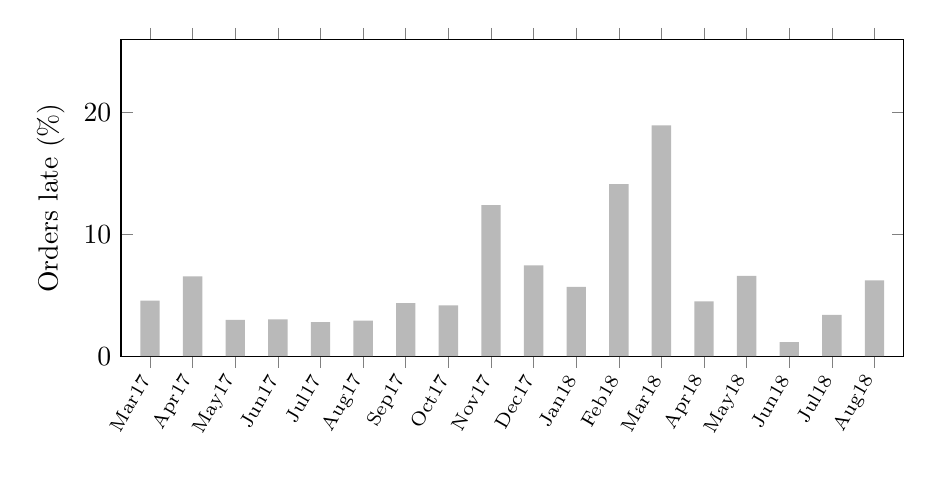
\begin{tikzpicture}
\begin{axis}[width=0.95\linewidth,height=5.6cm,ybar,bar width=7pt,ymin=0,ymax=26,ylabel={Orders late (\%)},
 symbolic x coords={Mar17,Apr17,May17,Jun17,Jul17,Aug17,Sep17,Oct17,Nov17,Dec17,Jan18,Feb18,Mar18,Apr18,May18,Jun18,Jul18,Aug18},xtick=data,x tick label style={rotate=60,anchor=east,font=\scriptsize},
 enlarge x limits=0.04]
\addplot[fill=gray!55,draw=none] coordinates {(Mar17,4.558) (Apr17,6.557) (May17,2.991) (Jun17,3.031) (Jul17,2.799) (Aug17,2.912) (Sep17,4.362) (Oct17,4.176) (Nov17,12.404) (Dec17,7.455) (Jan18,5.701) (Feb18,14.127) (Mar18,18.966) (Apr18,4.506) (May18,6.593) (Jun18,1.157) (Jul18,3.383) (Aug18,6.232)};
\end{axis}
\end{tikzpicture}
\caption{Share of orders late by purchase month. Black Friday (November 2017) and February--March 2018 stand out as the clearest swings in delivery conditions; the test period (June--August 2018, not shown) was calmer at \ClsTestLate{}\% late.}
\label{fig:monthly}
\end{figure}

\section*{Model 1: the two-stage delivery-time estimate (regression)}
\textbf{Method.} Both stages predict the same target, \texttt{delivery\_days}, so they are directly comparable and so a single success criterion applies: the handover update must beat the checkout estimate on the same orders in every validation window. The \textbf{checkout} stage uses the order, route and seller features known at purchase (20 inputs). The \textbf{handover} stage adds three inputs known once the carrier has the parcel: \texttt{handover\_days} (elapsed time), \texttt{approval\_days} (used only when approval was recorded by handover), and \texttt{route\_transit\_90d\_at\_handover} (the route's mean carrier-to-customer days over the previous 90 days, built only from deliveries already recorded, shrunk toward the all-route mean). Table~\ref{tab:ladder} shows each input's contribution with one fixed model (ridge, \(\alpha=100\)) so the gain is not confounded with model choice: most of the improvement comes from the elapsed time itself, consistent with the carrier leg's \CarrierShare{}\% share of delivery-time variance.

\begin{table}[ht]
\centering\small
\caption{Information ladder: ridge regression (\(\alpha=100\)) throughout, same orders at every rung, mean over five validation windows.}
\label{tab:ladder}
\begin{tabular}{@{}lrrr@{}}
\toprule
Rung & MAE (days) & \(R^2\) & Lowest-window \(R^2\) \\
\midrule
Checkout (20 frozen inputs) & \LadderCheckoutMAE{} & \LadderCheckoutRSq{} & \LadderCheckoutMinRSq{} \\
+ recent route transit history & \LadderTransitMAE{} & \LadderTransitRSq{} & \LadderTransitMinRSq{} \\
+ elapsed days to handover and approval & \LadderElapsedMAE{} & \LadderElapsedRSq{} & \LadderElapsedMinRSq{} \\
Handover (history as of handover) & \LadderHandoverMAE{} & \LadderHandoverRSq{} & \LadderHandoverMinRSq{} \\
\bottomrule
\end{tabular}
\end{table}

\textbf{Candidates and selection.} At each stage we compared the same line-up: a training-mean floor, Linear (plain, then ridge at three strengths) and Tree-based (plain decision tree, then depth-6 tree, random forest and two gradient-boosting settings) -- the handover stage also compares a rule baseline (elapsed days plus the route's recent transit average, no fitted model). We select the candidate with the lowest mean validation MAE, with ties broken by the paired one-standard-error rule: the simplest candidate whose mean gap to the best, over the five validation windows, is within one standard error of that gap~\cite{james2013}. This is standard in statistical learning (it is glmnet's default \texttt{lambda.1se}); the caveats are that we apply it across model families rather than within one penalty path (our simplicity order -- linear, then tree-based -- is a judgment call) and that the standard error comes from five non-independent windows.

At \textbf{checkout}, the random forest (\CheckoutBestName{}) has the lowest mean MAE (\CheckoutBestMAE{} days), but ridge \(\alpha=100\) is within one standard error (gap \CheckoutSelGap{} days, SE \CheckoutSelGapSE{}) and simpler, so it is selected (MAE \CheckoutSelMAE{}, RMSE \CheckoutSelRMSE{}, \(R^2\) \CheckoutSelRSq{}). At \textbf{handover}, ridge \(\alpha=100\) is both the lowest-MAE candidate and the one-SE selection (MAE \HandoverSelMAE{}, RMSE \HandoverSelRMSE{}, \(R^2\) \HandoverSelRSq{}); no simpler candidate's gap to it falls within one standard error. For reference, the handover rule baseline (elapsed days plus route average, no fitted model) scores MAE \HandoverRuleMAE{} and \(R^2\) \HandoverRuleRSq{}, close to the selected model: most of the signal is the elapsed time itself, and the fitted model adds a modest refinement. The training-mean floor scores MAE \CheckoutMeanMAE{} ($R^2$ \CheckoutMeanRSq{}) at both stages. We also tried an equal-weight voting ensemble of each family's best handover candidate (ridge and gradient boosting); at MAE 5.11 days it did not beat ridge alone, so ensembling was not adopted (\texttt{voting\_family\_winners}, Appendix~\ref{app:regression}). The full candidate table is in Appendix~\ref{app:regression}.

\begin{figure}[ht]
\centering
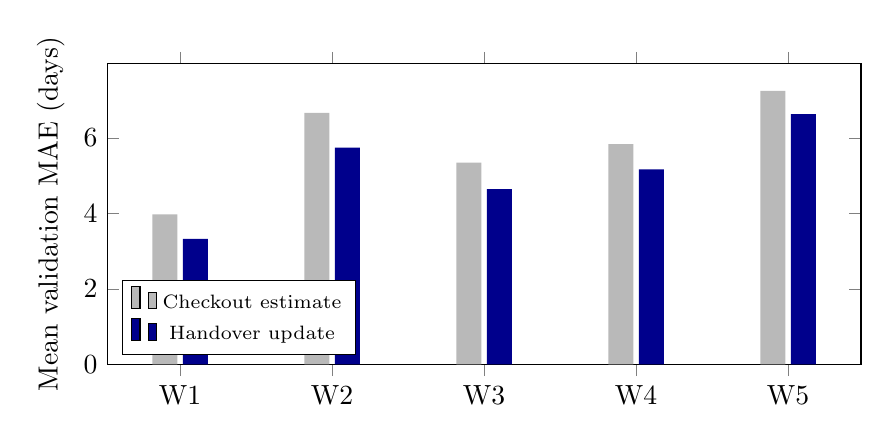
\begin{tikzpicture}
\begin{axis}[width=0.92\linewidth,height=5.4cm,ybar,bar width=9pt,ymin=0,ylabel={Mean validation MAE (days)},
 symbolic x coords={W1,W2,W3,W4,W5},xtick=data,enlarge x limits=0.12,legend style={at={(0.02,0.03)},anchor=south west,font=\scriptsize}]
\addplot[fill=gray!55,draw=none] coordinates {(W1,3.97) (W2,6.66) (W3,5.34) (W4,5.83) (W5,7.24)};
\addplot[fill=blue!55!black,draw=none] coordinates {(W1,3.32) (W2,5.74) (W3,4.64) (W4,5.16) (W5,6.63)};
\legend{Checkout estimate,Handover update}
\end{axis}
\end{tikzpicture}
\caption{Mean validation MAE by window, checkout estimate against the handover update (selected models). The handover update beats the checkout estimate in every window, including the higher-lateness windows.}
\label{fig:ladder}
\end{figure}

\textbf{Test results (post hoc).} The later test period was already open when the handover stage was designed, so these scores are reported as a post hoc check, not as the basis for selection. Checkout: MAE \CheckoutTestMAE{}, RMSE \CheckoutTestRMSE{}, \(R^2\) \CheckoutTestRSq{} (bias \CheckoutTestBias{} days, i.e.\ the model over-predicts, since the test period delivered faster than training). Handover: MAE \HandoverTestMAE{}, RMSE \HandoverTestRMSE{}, \(R^2\) \HandoverTestRSq{} (bias \HandoverTestBias{} days). The handover update's test \(R^2\) is positive while the checkout estimate's is negative, so moving the prediction point to handover also makes the estimate more robust to the regime shift between training and test, though it does not remove it.

\textbf{Same-period benchmark (secondary).} A random 5-fold validation and a random 20\% test from the saved secondary split give checkout \(R^2\) \CheckoutRandValRSq{} (validation) / \CheckoutRandTestRSq{} (test, MAE \CheckoutRandTestMAE{}) and handover \(R^2\) \HandoverRandValRSq{} (validation) / \HandoverRandTestRSq{} (test, MAE \HandoverRandTestMAE{}). These line up with public Olist models that use a held-out random split, which suggests the gap between our chronological \(R^2\) and higher published figures is mainly the evaluation design, not the model.

\textbf{What drives the estimate.} \CheckoutImpKind{}. At checkout the largest numeric/engineered coefficient is \texttt{\CheckoutImpAName{}} (\CheckoutImpAVal{}), then \texttt{\CheckoutImpBName{}} (\CheckoutImpBVal{}) and \texttt{\CheckoutImpCName{}} (\CheckoutImpCVal{}); customer-state dummies also carry large weights but are not individually interpretable as a ranked list. At handover, \texttt{\HandoverImpAName{}} (\HandoverImpAVal{}) is now the largest numeric/engineered coefficient -- the elapsed time itself -- ahead of \texttt{\HandoverImpBName{}} (\HandoverImpBVal{}) and \texttt{\HandoverImpCName{}} (\HandoverImpCVal{}), matching the ladder: once elapsed time is available, it dominates.

\section*{Model 2: the late warning (classification)}
\textbf{Method.} The classifier outputs the probability that an order misses Olist's promise, scored the moment the carrier takes the parcel. Candidates follow the same two families as the regression, tuned within each group (Linear: logistic regression over four regularisation strengths, with and without class weighting; Tree-based: a single tree, a random forest and gradient boosting, each over several depth/leaf settings), then compared with the plain-baseline-first line-up and the same paired one-standard-error rule~\cite{james2013}, scored by mean validation PR-AUC. The tuned forest (\ClsBestName{}) has the highest mean validation PR-AUC (\ValBestPR{}), but tuned logistic regression (\ClsSelName{}) is within one standard error (gap \ClsSelGap{}, SE \ClsSelGapSE{}) and simpler, so it is selected; it also clearly beats its own group's plain baseline (\ClsPlainName{}, PR-AUC \ClsPlainPR{}), so the tuning, not just the family choice, earns its place. The product is a ranking: each day operations works down the list from the top. The full candidate table is in Appendix~\ref{app:classifier}.

\textbf{Imbalance.} Only \ClsTestLate{}\% of test orders are late (4--21\% across the five validation windows), so accuracy is meaningless and a fixed 0.5 threshold would flag almost nothing. We report PR-AUC, which is more informative than ROC-AUC when positives are rare~\cite{saito2015}, against the late rate as the baseline, plus ROC-AUC, precision, recall, F1 and MCC at the chosen operating point.

\textbf{Operating point.} Because risk scores are not stable across periods, operations acts on a \emph{share} of each period's handovers rather than a fixed probability threshold. The share \(k\) is chosen on validation to maximise mean net benefit, valuing a caught late order at \BenefitRatio{} times the cost of acting on one order (a net-benefit calculation in the spirit of decision curve analysis~\cite{vickers2006}; this value is an assumption, not a measured cost). This gives \(k=\)\ActShare{}\%.

\begin{table}[ht]
\centering\small
\caption{Late warning on the test period, acting on the top \ActShare{}\% of orders by risk.}
\label{tab:classifier-test}
\begin{tabular}{@{}lcccccc@{}}
\toprule
& PR-AUC & ROC-AUC & Precision & Recall & F1 & MCC \\
\midrule
Late-warning model & \ClsTestPR{} & \ClsTestROC{} & \ClsTestPrec{}\% & \ClsTestRec{}\% & \ClsTestFone{} & \ClsTestMCC{} \\
Random list & \ClsTestLate{}\% & 0.50 & \ClsTestLate{}\% & \ActShare{}\% & --- & 0.00 \\
\bottomrule
\end{tabular}
\end{table}

Validation PR-AUC (\ValSelPR{}) is noticeably higher than test PR-AUC (\ClsTestPR{}); this tracks the late rate, not a validity problem: per-window PR-AUC rises and falls with the late rate (highest in the Black Friday and Feb--Mar windows, lowest in the calmest ones), and the test period was unusually calm (\ClsTestLate{}\% late, against 4--21\% in validation). ROC-AUC, which is less sensitive to the base rate, is \ClsTestROC{} on test against \ValSelROC{} on validation -- a smaller, more expected gap, and evidence that the ranking itself holds up; the net benefit at the validation-chosen \ActShare{}\% share was negative on the calm test period (\ClsNetBenefit{} per order), so the list should be sized to the current late rate rather than fixed in advance.

\begin{figure}[ht]
\centering
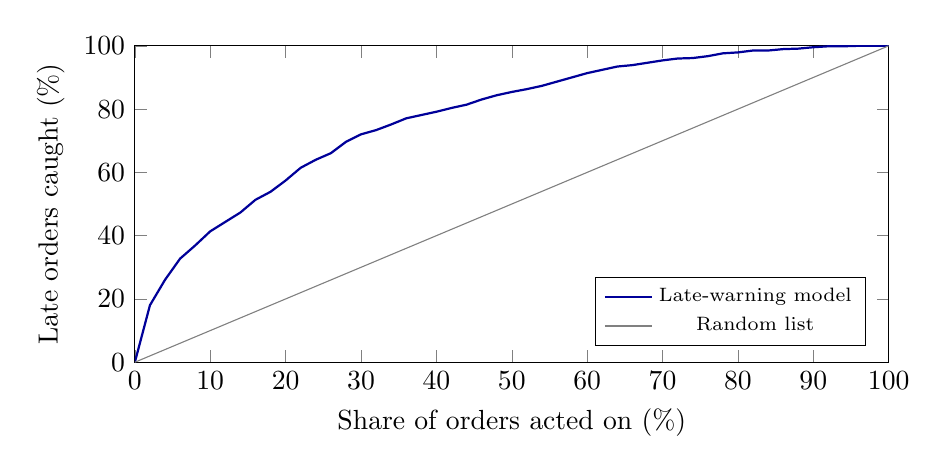
\begin{tikzpicture}
\begin{axis}[width=0.92\linewidth,height=5.6cm,xlabel={Share of orders acted on (\%)},ylabel={Late orders caught (\%)},
 xmin=0,xmax=100,ymin=0,ymax=100,legend style={at={(0.97,0.05)},anchor=south east,font=\scriptsize}]
\addplot[thick,blue!60!black,no marks] coordinates {(0.0,0.0000) (2.0,18.0060) (4.0,26.0417) (6.0,32.7381) (8.0,36.9048) (10.0,41.3690) (12.0,44.3452) (14.000000000000002,47.3214) (16.0,51.3393) (18.0,53.8690) (20.0,57.4405) (22.0,61.4583) (24.0,63.9881) (26.0,66.0714) (28.000000000000004,69.6429) (30.0,72.0238) (32.0,73.3631) (34.0,75.1488) (36.0,77.0833) (38.0,78.1250) (40.0,79.1667) (42.0,80.3571) (44.0,81.3988) (46.0,83.0357) (48.0,84.3750) (50.0,85.4167) (52.0,86.3095) (54.0,87.3512) (56.00000000000001,88.6905) (57.99999999999999,90.0298) (60.0,91.3690) (62.0,92.4107) (64.0,93.4524) (66.0,93.8988) (68.0,94.6429) (70.0,95.3869) (72.0,95.9821) (74.0,96.1310) (76.0,96.7262) (78.0,97.6190) (80.0,97.9167) (82.0,98.5119) (84.0,98.5119) (86.0,98.9583) (88.0,99.1071) (90.0,99.5536) (92.0,99.8512) (94.0,99.8512) (96.0,100.0000) (98.0,100.0000) (100.0,100.0000)};
\addlegendentry{Late-warning model}
\addplot[thin,gray,no marks] coordinates {(0.0,0.0000) (2.0,2.0000) (4.0,4.0000) (6.0,6.0000) (8.0,8.0000) (10.0,10.0000) (12.0,12.0000) (14.000000000000002,14.0000) (16.0,16.0000) (18.0,18.0000) (20.0,20.0000) (22.0,22.0000) (24.0,24.0000) (26.0,26.0000) (28.000000000000004,28.0000) (30.0,30.0000) (32.0,32.0000) (34.0,34.0000) (36.0,36.0000) (38.0,38.0000) (40.0,40.0000) (42.0,42.0000) (44.0,44.0000) (46.0,46.0000) (48.0,48.0000) (50.0,50.0000) (52.0,52.0000) (54.0,54.0000) (56.00000000000001,56.0000) (57.99999999999999,58.0000) (60.0,60.0000) (62.0,62.0000) (64.0,64.0000) (66.0,66.0000) (68.0,68.0000) (70.0,70.0000) (72.0,72.0000) (74.0,74.0000) (76.0,76.0000) (78.0,78.0000) (80.0,80.0000) (82.0,82.0000) (84.0,84.0000) (86.0,86.0000) (88.0,88.0000) (90.0,90.0000) (92.0,92.0000) (94.0,94.0000) (96.0,96.0000) (98.0,98.0000) (100.0,100.0000)};
\addlegendentry{Random list}
\end{axis}
\end{tikzpicture}
\caption{Cumulative share of late orders caught as operations works down the list, test period.}
\label{fig:gains}
\end{figure}

\textbf{Ranking quality.} The top 1\%, 5\%, 10\% and 20\% of the daily list contain \GainOneModel{}\%, \GainFiveModel{}\%, \GainTenModel{}\% and \GainTwentyModel{}\% of the late orders (Figure~\ref{fig:gains}); a random list contains 1\%, 5\%, 10\% and 20\%. On validation the top 10\% contained \ValSelRecallTen{}\% of late orders.

\textbf{What drives the score.} Permutation importance~\cite{breiman2001} (the drop in validation PR-AUC when a column is shuffled) is led by \texttt{\ImpAName{}} (\ImpADrop{}), then \texttt{\ImpBName{}} (\ImpBDrop{}) and \texttt{\ImpCName{}} (\ImpCDrop{}); all other inputs contribute under 0.02 each. The model is reading mainly how much of the promised time has already elapsed.

\begin{table}[ht]
\centering\small
\caption{Monthly test results for the late warning at the \ActShare{}\% share.}
\label{tab:classifier-monthly}
\begin{tabular}{@{}lrrrr@{}}
\toprule
Month & Orders & Late orders & Orders acted on & Late orders caught \\
\midrule
May (from the 26th) & \TestMayOrders{} & \TestMayLateCount{} & \TestMayActed{} & \TestMayCaught{} \\
June & \TestJunOrders{} & \TestJunLateCount{} & \TestJunActed{} & \TestJunCaught{} \\
July & \TestJulOrders{} & \TestJulLateCount{} & \TestJulActed{} & \TestJulCaught{} \\
August & \TestAugOrders{} & \TestAugLateCount{} & \TestAugActed{} & \TestAugCaught{} \\
\bottomrule
\end{tabular}
\end{table}

\section*{How Olist applies the models}
\begin{enumerate}\setlength{\itemsep}{0pt}
\item \textbf{At checkout}, the checkout-stage estimate sets the customer's expected delivery date.
\item \textbf{At handover}, every order gets an updated delivery-time estimate and a risk score; operations works down the day's ranked list from the top.
\item \textbf{For each flagged order}, the updated estimate shows how late it is likely to run: expedite with the carrier if there is still time to recover, otherwise proactively message the customer with a revised date.
\item \textbf{Ongoing}, both models are refit and the operating point (\(k\)) and candidate line-up are reviewed regularly, because delivery conditions shift (Figure~\ref{fig:monthly}) and a stale model or a fixed action share will drift out of step with them.
\end{enumerate}

\section*{Limitations and what we would do next}
\begin{itemize}\setlength{\itemsep}{0pt}
\item \textbf{Peaks are the hard case.} Both models were trained mostly on calmer months; validation includes the Black Friday and Feb--Mar 2018 windows specifically to test this, and the handover update and the classifier's ranking lift both hold up there, but with wider errors than in calm periods.
\item \textbf{Test period was calm.} At \ClsTestLate{}\% late, the test period understates how the late-warning model's net benefit behaves in a high-lateness month; operations should expect the \(k\) share and net benefit to need revisiting as conditions change, not treat the test numbers as a steady state.
\item \textbf{Cohort.} Results describe orders that were eventually delivered with a recorded carrier handover; cancelled and still-open orders have no outcome and are not covered.
\item \textbf{No causal claim.} We show that delivery time can be estimated and refined, and that late orders can be ranked, not that acting on either output improves customer experience or sales; a pilot with a control group would measure that.
\item \textbf{A calibrated promise buffer} (turning the checkout estimate into a promise with a chosen on-time rate, deployment detail only) was explored as a stretch goal; it is not part of this report's headline results.
\item \textbf{Next step.} Compare the late-warning ranking against the handover estimate's own implied lateness instead of only Olist's promise, as a clearly labelled simulation.
\end{itemize}

\appendix
\section{Full configuration tables}
\begin{table}[H]
\centering\small
\caption{Every regression candidate, mean over five validation windows.}
\label{tab:app-regression}
\begin{tabular}{@{}lllrrr@{}}
\toprule
Stage & Candidate & Family & MAE & RMSE & $R^2$ \\
\midrule
Checkout & mean\_baseline & mean & 7.215 & 10.671 & -0.078 \\
Checkout & linear\_baseline & linear & 5.860 & 9.464 & 0.155 \\
Checkout & ridge\_1 & ridge & 5.858 & 9.462 & 0.156 \\
Checkout & ridge\_10 & ridge & 5.848 & 9.451 & 0.158 \\
Checkout & ridge\_100 & ridge & 5.809 & 9.398 & 0.167 \\
Checkout & tree\_baseline & tree & 7.787 & 12.344 & -0.472 \\
Checkout & tree\_depth6 & tree & 5.933 & 9.505 & 0.144 \\
Checkout & forest\_leaf20 & forest & 5.783 & 9.340 & 0.176 \\
Checkout & boost\_baseline & boost & 5.830 & 9.452 & 0.155 \\
Checkout & boost\_slow & boost & 5.816 & 9.444 & 0.157 \\
Handover & mean\_baseline & mean & 7.215 & 10.671 & -0.078 \\
Handover & elapsed\_plus\_route\_baseline & rule & 5.304 & 8.396 & 0.337 \\
Handover & linear\_baseline & linear & 5.146 & 8.472 & 0.327 \\
Handover & ridge\_1 & ridge & 5.145 & 8.470 & 0.327 \\
Handover & ridge\_10 & ridge & 5.136 & 8.460 & 0.329 \\
Handover & ridge\_100 & ridge & 5.099 & 8.406 & 0.338 \\
Handover & tree\_baseline & tree & 6.840 & 11.625 & -0.330 \\
Handover & tree\_depth6 & tree & 5.313 & 8.633 & 0.299 \\
Handover & forest\_leaf20 & forest & 5.346 & 8.808 & 0.270 \\
Handover & boost\_baseline & boost & 5.214 & 8.651 & 0.297 \\
Handover & boost\_slow & boost & 5.215 & 8.666 & 0.294 \\
Handover & voting\_family\_winners & voting & 5.107 & 8.471 & 0.327 \\
\bottomrule
\end{tabular}
\end{table}
\label{app:regression}
\begin{table}[H]
\centering\small
\caption{Every classifier candidate, mean over five validation windows (handover stage).}
\label{tab:app-classifier}
\begin{tabular}{@{}lrrr@{}}
\toprule
Candidate & PR-AUC & ROC-AUC & Recall at top 10\% \\
\midrule
logistic\_c1 & 0.343 & 0.739 & 0.349 \\
logistic\_c1\_bal & 0.328 & 0.734 & 0.338 \\
logistic\_c0.01 & 0.367 & 0.769 & 0.363 \\
logistic\_c0.01\_bal & 0.350 & 0.761 & 0.350 \\
logistic\_c0.1 & 0.354 & 0.755 & 0.355 \\
logistic\_c0.1\_bal & 0.337 & 0.743 & 0.343 \\
logistic\_c10 & 0.338 & 0.733 & 0.345 \\
logistic\_c10\_bal & 0.325 & 0.730 & 0.335 \\
tree\_plain & 0.138 & 0.561 & 0.213 \\
tree\_d4\_l20 & 0.283 & 0.667 & 0.287 \\
tree\_d4\_l100 & 0.280 & 0.667 & 0.286 \\
tree\_d6\_l20 & 0.302 & 0.692 & 0.313 \\
tree\_d6\_l100 & 0.306 & 0.700 & 0.321 \\
tree\_d8\_l20 & 0.306 & 0.694 & 0.297 \\
tree\_d8\_l100 & 0.308 & 0.684 & 0.322 \\
tree\_d12\_l20 & 0.290 & 0.632 & 0.294 \\
tree\_d12\_l100 & 0.302 & 0.663 & 0.309 \\
forest\_l5\_sqrt & 0.360 & 0.735 & 0.338 \\
forest\_l5\_half & 0.344 & 0.723 & 0.319 \\
forest\_l20\_sqrt & 0.366 & 0.745 & 0.341 \\
forest\_l20\_half & 0.354 & 0.733 & 0.339 \\
forest\_l50\_sqrt & 0.369 & 0.747 & 0.343 \\
forest\_l50\_half & 0.357 & 0.737 & 0.344 \\
boost\_lr0.03\_n200\_l20 & 0.354 & 0.741 & 0.333 \\
boost\_lr0.03\_n200\_l100 & 0.345 & 0.739 & 0.329 \\
boost\_lr0.03\_n500\_l20 & 0.344 & 0.731 & 0.320 \\
boost\_lr0.03\_n500\_l100 & 0.333 & 0.729 & 0.318 \\
boost\_lr0.1\_n200\_l20 & 0.334 & 0.722 & 0.312 \\
boost\_lr0.1\_n200\_l100 & 0.330 & 0.719 & 0.309 \\
boost\_lr0.1\_n500\_l20 & 0.318 & 0.702 & 0.299 \\
boost\_lr0.1\_n500\_l100 & 0.318 & 0.703 & 0.300 \\
\bottomrule
\end{tabular}
\end{table}
\label{app:classifier}

\begin{thebibliography}{9}\small\setlength{\itemsep}{0pt}
\bibitem{bergmeir2012} C.~Bergmeir and J.~M.~Ben\'itez. On the use of cross-validation for time series predictor evaluation. \emph{Information Sciences}, 2012. doi:10.1016/j.ins.2011.12.028.
\bibitem{breiman2001} L.~Breiman. Random forests. \emph{Machine Learning}, 45(1):5--32, 2001.
\bibitem{james2013} G.~James, D.~Witten, T.~Hastie and R.~Tibshirani. \emph{An Introduction to Statistical Learning}, Sec.~6.1.3, p.~214. Springer, 2013.
\bibitem{saito2015} T.~Saito and M.~Rehmsmeier. The precision-recall plot is more informative than the ROC plot when evaluating binary classifiers on imbalanced datasets. \emph{PLOS ONE}, 10(3):e0118432, 2015.
\bibitem{salari2022} N.~Salari, S.~Liu and Z.-J.~M.~Shen. Real-time delivery time forecasting and promising in online retailing: when will your package arrive? \emph{Manufacturing \& Service Operations Management}, 24(3):1421--1436, 2022.
\bibitem{vickers2006} A.~J.~Vickers and E.~B.~Elkin. Decision curve analysis: a novel method for evaluating prediction models. \emph{Medical Decision Making}, 26(6):565--574, 2006.
\end{thebibliography}

\section*{Declaration on the use of AI}
We used Claude (Anthropic) as a coding and writing assistant for the Phase 2 analysis code, the figures and the first draft of this report. All numbers in this report are generated by \texttt{reports/phase2\_final\_evidence.py} from the saved results in \texttt{results/phase2/}. [Team to confirm before submission: that the team specified the design, reviewed the outputs, and takes responsibility for the content.]

\end{document}
